\section*{Dataset validation}
%Use section and subsection commands to organize your document. \LaTeX{}
%handles all the formatting and numbering automatically. Use ref and label
%commands for cross-references.

%This section is not essential for Web Tool papers. 
%For Data Articles, no analysis of the data, results or conclusions should be
%included and so this section should not be completed. 

\paragraph{Characters portraying emotions} Annotations for a total of
\AVTotalCharLabels\ and \AOTotalCharLabels\ different character categories were
created for the audio-visual movie (AV) and the audio movie (AO) respectively.
In the AV case, these comprise all possible characters but the narrator of the
audio-description.  There are \AVThreshCharLabels~(AV) and
\AOThreshCharLabels~(AO) characters for which there is a \AVAggThresh\ minimum
inter-rater agreement on the presence of a portrayed emotion for at least five
episodes of one second or longer throughout the entire movie (arbitrary
thresholds). The number of emotion episodes for the AV/AO union of these
characters sets is shown in figure \ref{fig:threshcharemo} (top).  As expected,
the majority of all portrayed emotions are associated with the main movie
characters Forrest, Dan, and Jenny.

\begin{figure*}
  \centering
  \includegraphics[trim=50 40 25 36,clip,width=\linewidth]{figures/character_episodes}\\
  \includegraphics[trim=50 40 25 36,clip,width=\linewidth]{figures/labeledemotion_episodes}
  \caption{Annotation frequencies by character and emotion. The minimum
    criterion for counting emotion episodes is a \AVAggThresh\ inter-observer agreement.
    Only categories/characters with a minimum of five such episodes are shown.
    The left panels show the number of episodes for both movie variants, the
    right panels show the commulative duration of emotion display across all
    considered episodes. The top panels show the annotation frequency by movie
    character, the bottom panels show the corresponding frequencies for emotion
  categories.}
  \label{fig:threshcharemo}
\end{figure*}

\paragraph{Portrayed emotion categories} For the audio movie
\AOFracWithLabeledEmotions\ of all annotations include at least one of the 22
explicit emotion label (see table \ref{tab:emotion_categories}), whereas only
\AVFracWithLabeledEmotions\ of annotations for the audio-visual movie contain
such a label. This is an indication that emotion cues in the visual movie more
diverse and ambiguous in comparison to the audio-only stimulus. Figure
\ref{fig:threshcharemo} (bottom) shows the frequency and display duration for
individual emotions. For both stimulus types the majority of all emotional
episodes involve the five categories anger/rage, fear, happiness, love and
sadness. Some of our pre-determined emotion categories have not been attributed
to any emotion episodes in the movie, or have been used very infrequently or
only by a small subset of observers.  Such emotions include resentment,
gratification, fears confirmed, or satisfaction (see table
\ref{tab:interobserver_consistency}).  It remains unknown whether these
emotions are not portrayed in the movie, or whether the respective categories
were not appropriately defined.

\paragraph{Emotion onset cues} Figure \ref{fig:threshlabeledoncue} shows the
frequency of individual emotion onset cues for all six distinguished cue types.
Only considering annotations with a minimum inter-rater agreement of
\AVAggThresh\ with respect to the type of onset cue, the two dominating emotion
cues are facial expressions (AV only) and verbal cues (for both stimulus
types), followed by gestures and body lanugage (AV only).
Figure~\ref{fig:indicatortsallchar} (bottom row) shows a rather uniform
distribution of verbal emotion cues across the entire duration of the movie for
both stimulus types. This suggests that a comparative analysis of verbal
emotion cue processing during AV~vs.~AO stimulation, as suggested above, may be
feasibile.

\begin{figure}
  \centering
  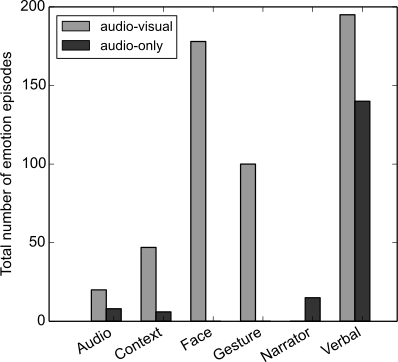
\includegraphics[trim=00 40 35 26,clip,width=\linewidth]{figures/labeledoncue_episodes}
  \caption{Number of emotion episodes for all distinguished onset cue categories
    (minimum \AVAggThresh\ inter-rater agreement) for both stimulus types.}
  \label{fig:threshlabeledoncue}
\end{figure}

\subsection*{Observer agreement as a probabilistic indicator}

It can be assumed that observers in this study have used individual intensity
thresholds for determining the start, end, or quality of an emotional episode.
Therefore, the IOA with respect to a particular aspect of
portrayed emotions at any given time in the movie could be seen as a measure of
the relative probability of perceiving an emotion feature. In order to assess
the reliability of such a measure, we generated time series for the
IOA with a sampling rate of \unit[1]{Hz}, as described above, and evaluated
their reliability and validity in terms of their correlation across observers,
stimulus types, and with each other.

\begin{figure*}
  \centering
  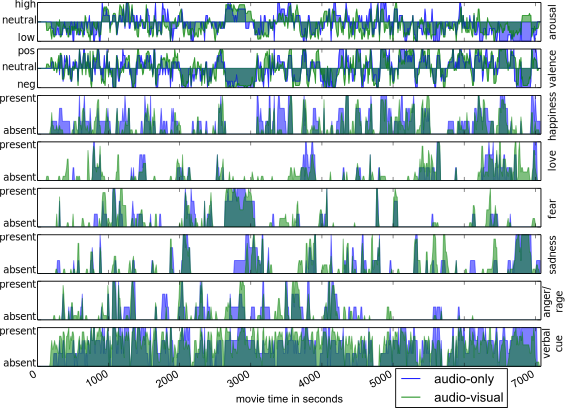
\includegraphics[trim=10 75 70 50,clip,width=\linewidth]{figures/indicator_ts_allchar}\\
  %includegraphics[width=\linewidth]{figures/indicator_ts_forrest}
  \caption{Inter-observer agreement (IOA) time courses for selected emotion
    attributes across the full duration of the movie. Extreme values indicate
    perfect agreement with respect to presence or absence of a particular emotion
    attribute at a given time. IOA time series for the two movie types are
    overlayed on top of each other.
    For the purpose of
    visualization the depicted time series reflects IOA computed using a
    \unit[10]{s} segment size, in contrast to \unit[1]{s} used for all other
  statistics presented in this paper.}
  \label{fig:indicatortsallchar}
\end{figure*}


\paragraph{Intra-stimulus inter-observer consistency}

The reliability of IOA time courses was estimated by
repeatedly splitting the set of observers into two groups of approximately
equal size. Within each group, IOA time courses where computed and correlated
across the observer sub-groups. Split-half correlations were computed for all
possible ways of combining observers into two groups (without replacement).
Table~\ref{tab:interobserver_consistency} shows the average time series
correlation across all splits, and the width of the 95\% confidence interval
of the mean.

In general, IOA reliability is larger for the AV movie annotations than for the
AO movie. This finding is likely a result of the lower number of observers for
latter. Intra-stimulus IOA reliability estimates suggest that a subset of
emotion attributes or categories is not contained in this AO movie stimulus,
the most prominent example is the direction of an emotion. Emotion categories
like hate, shame or relief also show large reliability differences between
stimulus type.  However, in these cases the small number of emotion episodes
may multiply the negative effect of the small number of observers on the
interpretability of this estimate.

Uniformly high reliability estimates were found for the two main dimensional
emotion attributes arousal and valence, as well as for the five most frequently
annotated emotion categories anger/rage, fear, happiness, love, and sadness.

\begin{table*}
  \centering
  \begin{tabular}{p{18mm}cccccc}
    & \multicolumn{2}{c}{\textbf{All characters}} & \multicolumn{2}{c}{\textbf{Forrest-only}} & \multicolumn{2}{c}{\textbf{Jenny-only}} \\
    & \textbf{Audio-visual} & \textbf{Audio-only} & \textbf{Audio-visual} & \textbf{Audio-only} & \textbf{Audio-visual} & \textbf{Audio-only} \\
    \\\hline\\
    \multicolumn{7}{l}{\textit{Dimensional emotion attributes}}\\
    Arousal & \AVInterRaterConsistArousalAllChar & \AOInterRaterConsistArousalAllChar & \AVInterRaterConsistArousalForrest & \AOInterRaterConsistArousalForrest & \AVInterRaterConsistArousalJenny & \AOInterRaterConsistArousalJenny \\
    Valence & \AVInterRaterConsistValenceAllChar & \AOInterRaterConsistValenceAllChar & \AVInterRaterConsistValenceForrest & \AOInterRaterConsistValenceForrest & \AVInterRaterConsistValenceJenny & \AOInterRaterConsistValenceJenny \\
    Direction & \AVInterRaterConsistDirectionAllChar & \AOInterRaterConsistDirectionAllChar & \AVInterRaterConsistDirectionForrest & \AOInterRaterConsistDirectionForrest & \AVInterRaterConsistDirectionJenny & \AOInterRaterConsistDirectionJenny \\
    \\\hline\\

    \multicolumn{7}{l}{\textit{Emotion categories}}\\
    Admiration     & \AVInterRaterConsistADMIRATIONAllChar     & \AOInterRaterConsistADMIRATIONAllChar     &\AVInterRaterConsistADMIRATIONForrest     &\AOInterRaterConsistADMIRATIONForrest     &\AVInterRaterConsistADMIRATIONJenny     &\AOInterRaterConsistADMIRATIONJenny     \\
    Anger/Rage     & \AVInterRaterConsistANGERRAGEAllChar      & \AOInterRaterConsistANGERRAGEAllChar      &\AVInterRaterConsistANGERRAGEForrest      &\AOInterRaterConsistANGERRAGEForrest      &\AVInterRaterConsistANGERRAGEJenny      &\AOInterRaterConsistANGERRAGEJenny      \\
    Compassion     & \AVInterRaterConsistCOMPASSIONAllChar     & \AOInterRaterConsistCOMPASSIONAllChar     &\AVInterRaterConsistCOMPASSIONForrest     &\AOInterRaterConsistCOMPASSIONForrest     &\AVInterRaterConsistCOMPASSIONJenny     &\AOInterRaterConsistCOMPASSIONJenny     \\
    Contempt       & \AVInterRaterConsistCONTEMPTAllChar       & \AOInterRaterConsistCONTEMPTAllChar       &\AVInterRaterConsistCONTEMPTForrest       &\AOInterRaterConsistCONTEMPTForrest       &\AVInterRaterConsistCONTEMPTJenny       &\AOInterRaterConsistCONTEMPTJenny       \\
    Disappoint. & \AVInterRaterConsistDISAPPOINTMENTAllChar & \AOInterRaterConsistDISAPPOINTMENTAllChar &\AVInterRaterConsistDISAPPOINTMENTForrest &\AOInterRaterConsistDISAPPOINTMENTForrest &\AVInterRaterConsistDISAPPOINTMENTJenny &\AOInterRaterConsistDISAPPOINTMENTJenny \\
    Fear           & \AVInterRaterConsistFEARAllChar           & \AOInterRaterConsistFEARAllChar           &\AVInterRaterConsistFEARForrest           &\AOInterRaterConsistFEARForrest           &\AVInterRaterConsistFEARJenny           &\AOInterRaterConsistFEARJenny           \\
    Fears conf.          & \AVInterRaterConsistFEARSCONFIRMEDAllChar           & \AOInterRaterConsistFEARSCONFIRMEDAllChar           &\AVInterRaterConsistFEARSCONFIRMEDForrest           &\AOInterRaterConsistFEARSCONFIRMEDForrest           &\AVInterRaterConsistFEARSCONFIRMEDJenny           &\AOInterRaterConsistFEARSCONFIRMEDJenny           \\
    Gloating       & \AVInterRaterConsistGLOATINGAllChar       & \AOInterRaterConsistGLOATINGAllChar       &\AVInterRaterConsistGLOATINGForrest       &\AOInterRaterConsistGLOATINGForrest       &\AVInterRaterConsistGLOATINGJenny       &\AOInterRaterConsistGLOATINGJenny       \\
    Gratification  & \AVInterRaterConsistGRATIFICATIONAllChar  & \AOInterRaterConsistGRATIFICATIONAllChar  &\AVInterRaterConsistGRATIFICATIONForrest  &\AOInterRaterConsistGRATIFICATIONForrest  &\AVInterRaterConsistGRATIFICATIONJenny  &\AOInterRaterConsistGRATIFICATIONJenny  \\
    Gratitude      & \AVInterRaterConsistGRATITUDEAllChar      & \AOInterRaterConsistGRATITUDEAllChar      &\AVInterRaterConsistGRATITUDEForrest      &\AOInterRaterConsistGRATITUDEForrest      &\AVInterRaterConsistGRATITUDEJenny      &\AOInterRaterConsistGRATITUDEJenny      \\
    Happiness      & \AVInterRaterConsistHAPPINESSAllChar      & \AOInterRaterConsistHAPPINESSAllChar      &\AVInterRaterConsistHAPPINESSForrest      &\AOInterRaterConsistHAPPINESSForrest      &\AVInterRaterConsistHAPPINESSJenny      &\AOInterRaterConsistHAPPINESSJenny      \\
    Happy-for      & \AVInterRaterConsistHAPPYFORAllChar       & \AOInterRaterConsistHAPPYFORAllChar       &\AVInterRaterConsistHAPPYFORForrest       &\AOInterRaterConsistHAPPYFORForrest       &\AVInterRaterConsistHAPPYFORJenny       &\AOInterRaterConsistHAPPYFORJenny       \\
    Hate           & \AVInterRaterConsistHATEAllChar           & \AOInterRaterConsistHATEAllChar           &\AVInterRaterConsistHATEForrest           &\AOInterRaterConsistHATEForrest           &\AVInterRaterConsistHATEJenny           &\AOInterRaterConsistHATEJenny           \\
    Hope           & \AVInterRaterConsistHOPEAllChar           & \AOInterRaterConsistHOPEAllChar           &\AVInterRaterConsistHOPEForrest           &\AOInterRaterConsistHOPEForrest           &\AVInterRaterConsistHOPEJenny           &\AOInterRaterConsistHOPEJenny           \\
    Love           & \AVInterRaterConsistLOVEAllChar           & \AOInterRaterConsistLOVEAllChar           &\AVInterRaterConsistLOVEForrest           &\AOInterRaterConsistLOVEForrest           &\AVInterRaterConsistLOVEJenny           &\AOInterRaterConsistLOVEJenny           \\
    Pride          & \AVInterRaterConsistPRIDEAllChar          & \AOInterRaterConsistPRIDEAllChar          &\AVInterRaterConsistPRIDEForrest          &\AOInterRaterConsistPRIDEForrest          &\AVInterRaterConsistPRIDEJenny          &\AOInterRaterConsistPRIDEJenny          \\
    Relief         & \AVInterRaterConsistRELIEFAllChar         & \AOInterRaterConsistRELIEFAllChar         &\AVInterRaterConsistRELIEFForrest         &\AOInterRaterConsistRELIEFForrest         &\AVInterRaterConsistRELIEFJenny         &\AOInterRaterConsistRELIEFJenny         \\
    Remorse        & \AVInterRaterConsistREMORSEAllChar        & \AOInterRaterConsistREMORSEAllChar        &\AVInterRaterConsistREMORSEForrest        &\AOInterRaterConsistREMORSEForrest        &\AVInterRaterConsistREMORSEJenny        &\AOInterRaterConsistREMORSEJenny        \\
    Resentment     & \AVInterRaterConsistRESENTMENTAllChar     & \AOInterRaterConsistRESENTMENTAllChar     &\AVInterRaterConsistRESENTMENTForrest     &\AOInterRaterConsistRESENTMENTForrest     &\AVInterRaterConsistRESENTMENTJenny     &\AOInterRaterConsistRESENTMENTJenny     \\
    Sadness        & \AVInterRaterConsistSADNESSAllChar        & \AOInterRaterConsistSADNESSAllChar        &\AVInterRaterConsistSADNESSForrest        &\AOInterRaterConsistSADNESSForrest        &\AVInterRaterConsistSADNESSJenny        &\AOInterRaterConsistSADNESSJenny        \\
    Satisfaction   & \AVInterRaterConsistSATISFACTIONAllChar   & \AOInterRaterConsistSATISFACTIONAllChar   &\AVInterRaterConsistSATISFACTIONForrest   &\AOInterRaterConsistSATISFACTIONForrest   &\AVInterRaterConsistSATISFACTIONJenny   &\AOInterRaterConsistSATISFACTIONJenny   \\
    Shame          & \AVInterRaterConsistSHAMEAllChar          & \AOInterRaterConsistSHAMEAllChar          &\AVInterRaterConsistSHAMEForrest          &\AOInterRaterConsistSHAMEForrest          &\AVInterRaterConsistSHAMEJenny          &\AOInterRaterConsistSHAMEJenny          \\\\                  
    \hline\\
    \multicolumn{7}{l}{\textit{Emotion onset cues}}\\
    Audio & \AVInterRaterConsistAUDIOAllChar &\AOInterRaterConsistAUDIOAllChar &\AVInterRaterConsistAUDIOForrest &\AOInterRaterConsistAUDIOForrest &\AVInterRaterConsistAUDIOJenny &\AOInterRaterConsistAUDIOJenny \\
    Context & \AVInterRaterConsistCONTEXTAllChar & \AOInterRaterConsistCONTEXTAllChar &\AVInterRaterConsistCONTEXTForrest &\AOInterRaterConsistCONTEXTForrest &\AVInterRaterConsistCONTEXTJenny &\AOInterRaterConsistCONTEXTJenny \\
    Face & \AVInterRaterConsistFACEAllChar & \AOInterRaterConsistFACEAllChar &\AVInterRaterConsistFACEForrest &\AOInterRaterConsistFACEForrest &\AVInterRaterConsistFACEJenny &\AOInterRaterConsistFACEJenny \\
    Gesture & \AVInterRaterConsistGESTUREAllChar & \AOInterRaterConsistGESTUREAllChar &\AVInterRaterConsistGESTUREForrest &\AOInterRaterConsistGESTUREForrest &\AVInterRaterConsistGESTUREJenny &\AOInterRaterConsistGESTUREJenny \\
    Narrator & \AVInterRaterConsistNARRATORAllChar & \AOInterRaterConsistNARRATORAllChar &\AVInterRaterConsistNARRATORForrest  &\AOInterRaterConsistNARRATORForrest &\AVInterRaterConsistNARRATORJenny &\AOInterRaterConsistNARRATORJenny \\
    Verbal & \AVInterRaterConsistVERBALAllChar & \AOInterRaterConsistVERBALAllChar &\AVInterRaterConsistVERBALForrest  &\AOInterRaterConsistVERBALForrest &\AVInterRaterConsistVERBALJenny &\AOInterRaterConsistVERBALJenny \\
    \\\hline
 

%    \multicolumn{7}{l}{\textit{Intra-stimulus indicator correlation}} \\\\
%    Arousal-Valence & \AVCorrArousalValenceAllChar & \AOCorrArousalValenceAllChar & \AVCorrArousalValenceForrest & \AOCorrArousalValenceForrest & \AVCorrArousalValenceJenny & \AOCorrArousalValenceJenny \\
%    Arousal-Direction & \AVCorrArousalDirectionAllChar & \AOCorrArousalDirectionAllChar & \AVCorrArousalDirectionForrest & \AOCorrArousalDirectionForrest & \AVCorrArousalDirectionJenny & \AOCorrArousalDirectionJenny \\
%    Valence-Direction & \AVCorrValenceDirectionAllChar & \AOCorrValenceDirectionAllChar & \AVCorrValenceDirectionForrest & \AOCorrValenceDirectionForrest & \AVCorrValenceDirectionJenny & \AOCorrValenceDirectionJenny \\
%    \\\hline\\
  \end{tabular}

  \caption{
    Intra-stimulus inter-observer consistency. All values are Pearson
    correlation coefficients for \unit[1]{Hz} modulations of the fraction of
    IOA (as, for example, depicted in figure
    \ref{fig:indicatortsallchar}) with respect to a particular emotion
    attribute across the entire duration of the movie. The specified range
    corresponds to the width of the 95\% confidence interval of the mean correlation
    for all possible combinations of partitioning observers into two sub-groups (audio-visual
    4~vs.~5; audio-only 1~vs~2). Higher correlations indicate higher consistency
    of aggreement modulations across observer sub-groups.
    The \textit{all characters} column indicates the agreement for a particular
    emotion attribute over time irrespective of the annotated character. The
    columns on the right show the corresponding correlations for the two main
    characters. \textit{n/a} fields indicate an insufficient number of annotation to compute
    the consistency measure.}
  \label{tab:interobserver_consistency}
\end{table*}

\paragraph{Intra-stimulus inter-variable correlations}

In order to assess possible confounds in the annotations, we computed the
correlation of intra-stimulus IOA time courses (across all observers) for all
pairwise combinations of emotion attributes and categories. The correlation
matrices for the AV and the AO movie stimulus are depicted in figure
\ref{fig:intrastimcorrelation}. The results reveal an expected correlation
pattern between individual emotion categories and the two main dimensional
attributes arousal and valence, with stronger correlations being observed for
more primary and more frequently portrayed emotions. Interestingly, audio and
verbal cues in the AV stimulus seems to be more associated with a high state
of arousal and emotions directed towards other people than in the AO stimulus.
In the AV stimulus facial expressions seem to have a tendency to communicate
negative emotions, rather than positive ones.


\begin{figure*}
  \centering
  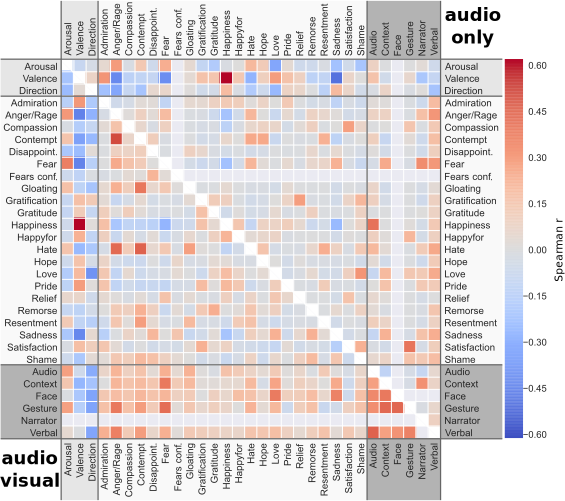
\includegraphics[width=\linewidth]{figures/bigcorr}
  \caption{Intra-stimulus indicator correlation. The lower triangular matrix
    depicts the correlations between the IOA time courses for
    the three primary bipolar emotion attributes (arousal [high/low], valence [pos/neg], and direction [self/other]), the
    22 emotion categories, and the six emotion onset indicators for the audio-visual
    movie. The upper triangular matrix shows the corresponding correlations for the
    audio-only movie.
 }
  \label{fig:intrastimcorrelation}
\end{figure*}

\paragraph{Inter-stimulus consistency}

To estimate the similarity of the two stimulus types, we computed the
correlation of IOA time courses for the AV and the AO movie with respective
to emotion attributes and categories. Table~\ref{tab:interstim_consistency}
shows the respective correlations and their 95\% confidence interval. Again,
the three dimensional attributes, as well as the five most frequent emotion
categories show significant correlations. This is evidence for an expected
substantial semantic similarity with respected to the emotional content in the
two variants of the ``Forrest Gump'' movie.

\begin{table*}
  \centering
  \begin{tabular}{p{26mm}ccc}
    & \textbf{All characters} & \textbf{Forrest-only} & \textbf{Jenny-only} \\
    \hline \\
    \multicolumn{4}{l}{\textit{Dimensional emotion attributes}}\\
    Arousal & \InterModCorrArousalAllChar &\InterModCorrArousalForrest &\InterModCorrArousalJenny \\
    Valence & \InterModCorrValenceAllChar &\InterModCorrValenceForrest &\InterModCorrValenceJenny \\
    Direction & \InterModCorrDirectionAllChar &\InterModCorrDirectionForrest &\InterModCorrDirectionJenny \\\\\hline\\

    \multicolumn{4}{l}{\textit{Emotion categories}}\\
    Admiration & \InterModCorrADMIRATIONAllChar &\InterModCorrADMIRATIONForrest &\InterModCorrADMIRATIONJenny \\
    Anger/Rage & \InterModCorrANGERRAGEAllChar &\InterModCorrANGERRAGEForrest &\InterModCorrANGERRAGEJenny \\
    Compassion & \InterModCorrCOMPASSIONAllChar &\InterModCorrCOMPASSIONForrest &\InterModCorrCOMPASSIONJenny \\
    Contempt & \InterModCorrCONTEMPTAllChar &\InterModCorrCONTEMPTForrest &\InterModCorrCONTEMPTJenny \\
    Disappointment & \InterModCorrDISAPPOINTMENTAllChar &\InterModCorrDISAPPOINTMENTForrest &\InterModCorrDISAPPOINTMENTJenny \\
    Fear & \InterModCorrFEARAllChar &\InterModCorrFEARForrest &\InterModCorrFEARJenny \\
    Gloating & \InterModCorrGLOATINGAllChar &\InterModCorrGLOATINGForrest &\InterModCorrGLOATINGJenny \\
    Gratification & \InterModCorrGRATIFICATIONAllChar &\InterModCorrGRATIFICATIONForrest &\InterModCorrGRATIFICATIONJenny \\
    Gratitude & \InterModCorrGRATITUDEAllChar &\InterModCorrGRATITUDEForrest &\InterModCorrGRATITUDEJenny \\
    Happiness & \InterModCorrHAPPINESSAllChar &\InterModCorrHAPPINESSForrest &\InterModCorrHAPPINESSJenny \\
    Happy-for & \InterModCorrHAPPYFORAllChar &\InterModCorrHAPPYFORForrest &\InterModCorrHAPPYFORJenny \\
    Hate & \InterModCorrHATEAllChar &\InterModCorrHATEForrest &\InterModCorrHATEJenny \\
    Hope & \InterModCorrHOPEAllChar &\InterModCorrHOPEForrest &\InterModCorrHOPEJenny \\
    Love & \InterModCorrLOVEAllChar &\InterModCorrLOVEForrest &\InterModCorrLOVEJenny \\
    Pride & \InterModCorrPRIDEAllChar &\InterModCorrPRIDEForrest &\InterModCorrPRIDEJenny \\
    Relief & \InterModCorrRELIEFAllChar &\InterModCorrRELIEFForrest &\InterModCorrRELIEFJenny \\
    Remorse & \InterModCorrREMORSEAllChar &\InterModCorrREMORSEForrest &\InterModCorrREMORSEJenny \\
    Resentment & \InterModCorrRESENTMENTAllChar &\InterModCorrRESENTMENTForrest &\InterModCorrRESENTMENTJenny \\
    Sadness & \InterModCorrSADNESSAllChar &\InterModCorrSADNESSForrest &\InterModCorrSADNESSJenny \\
    Satisfaction & \InterModCorrSATISFACTIONAllChar &\InterModCorrSATISFACTIONForrest &\InterModCorrSATISFACTIONJenny \\
    Shame & \InterModCorrSHAMEAllChar &\InterModCorrSHAMEForrest &\InterModCorrSHAMEJenny \\
    \\\hline\\
    \multicolumn{4}{l}{\textit{Emotion onset cues}}\\
    Audio & \InterModCorrAUDIOAllChar &\InterModCorrAUDIOForrest &\InterModCorrAUDIOJenny \\
    Context & \InterModCorrCONTEXTAllChar &\InterModCorrCONTEXTForrest &\InterModCorrCONTEXTJenny \\
    %Face & \InterModCorrFACEAllChar &\InterModCorrFACEForrest &\InterModCorrFACEJenny \\
    %Gesture & \InterModCorrGESTUREAllChar &\InterModCorrGESTUREForrest &\InterModCorrGESTUREJenny \\
    %Narrator & \InterModCorrNARRATORAllChar &\InterModCorrNARRATORForrest &\InterModCorrNARRATORJenny \\
    Verbal & \InterModCorrVERBALAllChar &\InterModCorrVERBALForrest &\InterModCorrVERBALJenny \\
    \\\hline

  \end{tabular}

  \caption{ Inter-stimulus indicator correlation. All values are Pearson
    correlation coefficients of \unit[1]{Hz} modulations of the fraction of
    IOA (as, for example, depicted in figure
    \ref{fig:indicatortsallchar}) for the two stimulus types (audio-visual and
  audio-only movie). The specified range corresponds to the width of the 95\%
confidence interval of correlation coefficient (computed via Fisher
transformation).}


  \label{tab:interstim_consistency}
\end{table*}

\hl{TODO: are there annotations that do not contain indicators specifications?

Current: \AVFracWithLabeledOncue \AOFracWithLabeledOncue
}

